\section{Backend}
%TODO: @Joshua

\subsection{Aufbau}

Der Aufbau der Serverapplikation orientiert sich am Konzept der Onion-Architecture.
In Onion Architecture wird die Applikation in Layer aufgeteilt.

\begin{figure}[h]
    \centering
    \begin{minipage}[b]{0.4\textwidth}
        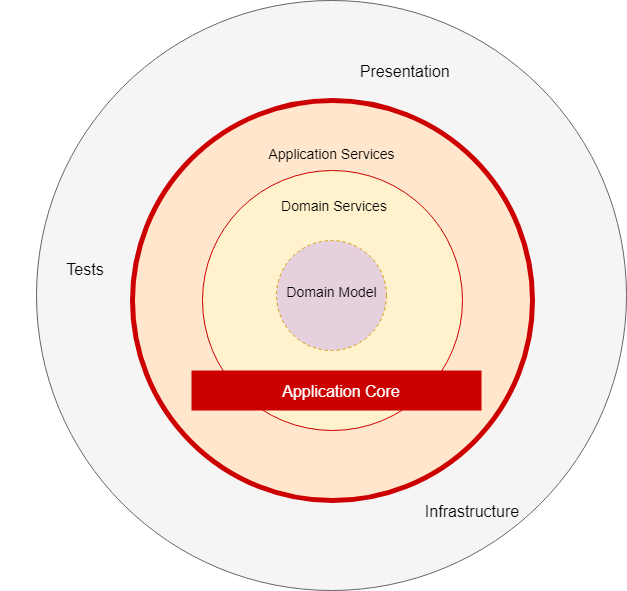
\includegraphics[width=\textwidth]{graphics/thinktocode-onion}
        \caption{Onion Architecture}
    \end{minipage}
\end{figure}

Um zu garantieren, dass keine ungewollten Abhängigkeiten zwischen Layern bestehen, können die Layers in eigene Module verpackt werden.
Dies erhöht jedoch die interne Komplexität der Applikation.
Die Umsetzung wird aufgrund der geringen Projektgrösse deshalb nicht in unabhängigen Modulen realisiert, sondern über die Package Struktur angedeutet.

Bei der Implementation wird dabei konsequent darauf geachtet, die einzelnen Layer so zu halten das diese als eigenständige Module extrahiert werden können.
Für die Verwaltung der Komponenten der Serverapplikation wird folgende Packagestruktur definiert:

\begin{figure}[h]
    \centering
    \begin{minipage}[b]{0.9\textwidth}
        \dirtree{%
            .1 ch.fhnw.woweb.teamdocumentserver.
            .2 api.
            .2 config.
            .2 domain.
            .2 persistence.
            .2 service.
            .2 web.
        }
        \caption{Package Struktur Cloud Service}\label{fig:packagescloudservice}
    \end{minipage}
\end{figure}


Im Zentrum des Modells steht der Domain Layer.
Dieser beinhaltet die Domänenobjekte und darf nur Abhängigkeiten auf sich selbst haben.
Umgekehrt dürfen aber alle anderen Layers Abhängigkeiten auf den Domain Layer haben.
Der Domain Layer wird mit dem Package domain abgebildet.

Die nächste Schicht im Modell ist der Domain Service Layer.
Dieser bietet die fachliche Logik und definiert die Verhaltensweise des Domain Layers.
Der Layer Application Services bildet die Brücke zwischen externer Infrastruktur und Domain Services.
Dies beinhaltet Repository Services für die Schnittstelle zu persistentem Speicher und Rest Controllers für Schnittstellen zu anderen Applikationen.
In der äussersten Schicht steht der Infrastructure Layer.
Dieser beinhaltet externe Systeme, welche von der Applikation benötigt werden wie Datenbank und Benutzeroberfläche.






Im Zentrum steht das Package Domäne.
Es beinhaltet alle Domänenobjekte und stellt alleine den Domäne Layer dar.

Der Domain Service Layer wird durch das Package Service abgebildet.
Hier werden sämtliche Domain Services implementiert.
Die Packages persistence und web beinhalten schliesslich den Application Service Layer.
Dabei definiert das Package persistence Services welche für Interaktion mit der Datenbank verwendet werden.
Das Package web definiert die HTTP-Endpunkte, welche für die Kommunikation mit dem Frontend des Systems verwendet werden.
Diese werden im Package services implementiert und im package Web verwendet.
Letztlich beinhaltet das Package config die technische Konfiguration der Applikation.




\subsection{API}

\subsection{Komponenten}

\subsection{Sequenz}

\subsection{State- und Konfliktmanagment}
